% include the figures path relative to the master file
% \graphicspath{ {./content/method/figures/visual_cues/}{./content/method/figures/}}
\graphicspath{ {./content/method/figures/}}

\section{Materials and Methods}\label{sec:method}
\todo{Mention texture here, rework where the sections are called}


%\subsection{Experimental Framework description}

The proposed method, as well as, its experimental set-up for \ac{oct} volume classification are outlined in Fig.\,\ref{fig:ML-scheme}.
%The methodology is formulated as a standard classification procedure.
The methodology is formulated as a standard classification procedure, through 5 steps.
First, the \ac{oct} volumes are pre-processed as presented in details in Sect.\,\ref{subsec:prepro}.
The mapping stage is used to determine a discrete set of elements (or structures) which is used for representing the \ac{oct} volume.
For this work two mapping strategies are defined: (i) \emph{global} and (ii) \emph{local} mapping.
In the global mapping approach, a single structure is computed for the image/volume while in the local mapping, a set of structures is defined by sliding a window through the image/volume.
Then, a descriptor is computed for each structure.
The feature extraction and representation are presented in depth in Sect.\,\ref{subsec:feaext} and Sect.\,\ref{subsec:fearep}, respectively.
Finally the classification step is presented in Sect.\,\ref{subsec:cls}.
%A \ac{rf} classifier has been selected to perform the classification of the \ac{oct} volume~\cite{breiman2001random}.

% \subsection{Data}
% \color{red}{
%   \begin{itemize}
%   \item cross-validation
%   \item our dataset
%   \item DUC dataset
%   \end{itemize}}\color{black}

% For evaluation purposes, the results have been cross-validated, by splitting the data in training and testing using a \ac{lopo} strategy. In this manner for each round a pair \color{red}{dce,normal} has been selected to be used as the round test set, while the rest of the dataset has been used as a training. \color{red}{Doing the cross validation in this manner, has the limitation that despite the fact that the results are robust due to the cross validation, no results variance can be reported. However, and despite this limitation, \ac{lopo} has been choose due to the reduced amount of \ac{oct} volumes available.}\color{black}


\subsection{Image pre-processing}\label{subsec:prepro}

This section describes set of pre-processing techniques which are provided by our framework.
These approaches can be arbitrarily combined.
Combinations of these technologies and the influence of these combinations are reported in experimentation~\cref{sec:exp}.

\subsubsection{\acf{nlm}}
\Ac{oct} images are known to be affected by a speckle noise~\cite{schmitt1999speckle}.
Subsequently, \ac{nlm}~\cite{buades2005non} filtering has been successfully used in \ac{us} images to filter similar noise~\cite{Coupe2009} and is used in our framework to denoise each B-scan (i.e. each $x-z$ slice) of the \ac{oct} volumes (see in Fig.\,\ref{subfig:vol}).
\added[id = moj]{In this regard (For this reason, Due to this reason), we use the \ac{nlm} filtering which has been successfully used on \ac{us} images to remove similar noise~\cite{Coupe2009}.
This filter is applied on each B-scan (i.e. each $x-z$ slice) for the \ac{oct} volumes (see in Fig.\,\ref{subfig:vol}).}
%The pre-processing stage in the proposed methodology applies an image denoising method to reduce the speckle noise in \ac{oct} images.
%Since image details and texture of the original image are needed by the following stages in the method, \ac{nlm} algorithm \cite{buades2005non} is used.
\ac{nlm} filtering offers the advantage to use all the possible self-predictions that the image can provide rather than local or frequency filters such as Gaussian, anisotropic or Wiener filters~\cite{buades2005non}.
An example of filtering using \ac{nlm} filter on \ac{oct} image is depicted in Fig\,\ref{subfig:raw} and Fig.\,\ref{subfig:nlm}.

\begin{figure}[t]
  \centering
  \hspace*{\fill}
  \subfigure[]{\label{subfig:vol}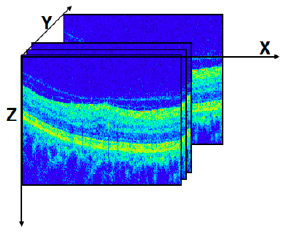
\includegraphics[width=0.3\linewidth]{volume.png}} \hfill
  \subfigure[]{\label{subfig:raw}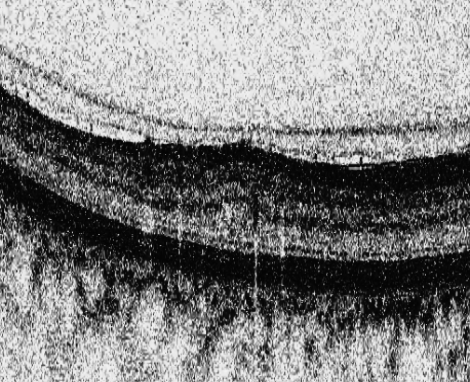
\includegraphics[width=0.3\linewidth]{raw_crop_grey.png}} \hfill
  \subfigure[]{\label{subfig:nlm}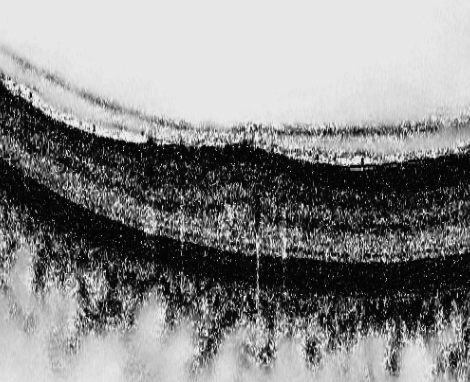
\includegraphics[width=0.3\linewidth]{nlm_crop_grey.png}}
  \hspace*{\fill}
  \caption{\ac{oct}: (a) Organization of the \ac{oct} data - (b) Original image - (c) \ac{nlm} filtering.}
  \label{fig:denoise}
\end{figure}

\subsubsection{Flatten}

Texture descriptors characterize spatial arrangement of intensities.
Therefore, to ensure a consistent characterization of the tissue disposition regardless of the location within the retina, the natural curvature of the retina needs to be taken into account.
This can be done in different manners:
\begin{itemize}
    \item using a descriptor allowing for a wide number of textures, so that
      each texture orientation accounts for each own descriptor.
    \item using a rotation invariant descriptor.
    \item by unfolding the curvature of the retina.
\end{itemize}

This process of unfolding the curvature of the retina is known as image flattening. When flattening, an estimation of the \rpe  layer is used to modify the volume by imposing that the \rpe  should be flat.
Our implementation modifies the proposal of Liu\,\textit{et al.}~\cite{Liu2011}, as illustrated in \Cref{fig:flatten}. Othsu thresholding is used to segment the retina from the background. A line is fitted to the bottom part of the segmentation hull, since it is assumed to be parallel to the \rpe. The image is corrected based on this line.

\begin{figure}[t]
  \missingfigure{Illustration of (a) orignail image, (b) segmentation, (c) feeting curve, flattening, (d) corrected image}
  \caption{}
  \label{fig:flatten}
\end{figure}


\subsubsection{Slice alignment}
Similarly, when using 3D texture, misalignment between the slice introduce error to the texture descriptor. In this case the slices are also aligned based on the segmentation's hull.

\subsubsection{Background cropping}
\todo[inline]{Cropping out the background allows for less texture to be encoded}

\subsection{Features extraction}\label{subsec:feaext}
\todo[inline]{This a generic description. Shall we place it for our images with some picture? (maybe we don't have time)}
\added[id=moj]{In this research we chose to extract simple and efficient \ac{lbp} texture features with regards to each \ac{oct} slice and volumes.}
\ac{lbp} is a texture descriptor based on the signs of the differences of a central pixel with respect to its neighboring pixels~\cite{ojala2002multiresolution}.
%More precisely, this descriptor encodes the intensity differences of a central pixel ($g_c$) with its neighboring pixels ($g_{p}$), within in a defined neighborhood of radius $R$.
These differences are encoded in terms of binary patterns as in~Eq.\,\eqref{Eq:LBP}:

\begin{equation}\label{Eq:LBP}
LBP_{P,R} = \sum_{p=0}^{P-1}s(g_{p} - g_{c})2^{p} \ , \qquad s(\cdot) = \begin{cases}
    1  & \ \text{if } (g_{p} - g_{c}) \geq 0\\
    0  & \ \text{otherwise}\\
  \end{cases} \ ,
\end{equation}

% \begin{align} \label{Eq:LBP}
% LBP_{P,R} = \sum_{p=0}^{P-1}s(g_{p} - g_{c})2^{p}& \ , \\
% \text{where } &s(\cdot) = \begin{cases}
%     1  & \quad \text{if } g_{p} - g_{c} \geq 0\\
%     0  & \quad \text{otherwise}\nonumber\\
%   \end{cases} \ .
% \end{align}
\noindent where $g_c$, $g_{p}$ are the intensities of the central pixel and a given neighbor pixel, respectively. $P$ is the number of sampling points in the circle of radius $R$. Figure~\ref{subfig:lbp} illustrates the meaning of $P$ and $R$.

\begin{changebar}
\todo{Are we doing Rotation Invariant version??}
Ojala\,\textit{et al.} further extend the original \ac{lbp} formulation to achieve rotation invariance at the expense of limiting the texture description to the notion of circular ``uniformity''~\cite{ojala2002multiresolution}.
\end{changebar}
Volume encoding is later proposed by Zhao\,\textit{et al.} by computing \ac{lbp} descriptors in each orthogonal planes, so called \ac{lbptop}~\cite{zhao2012rotation}.

\begin{figure}[t]
  \centering
  \hspace*{\fill}
  \subfigure[]{\label{subfig:lbp}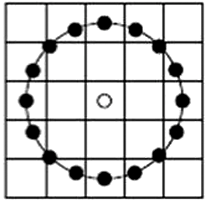
\includegraphics[height=0.1\textheight]{lbp.png}} \hfill
  \subfigure[]{\label{subfig:lbptop}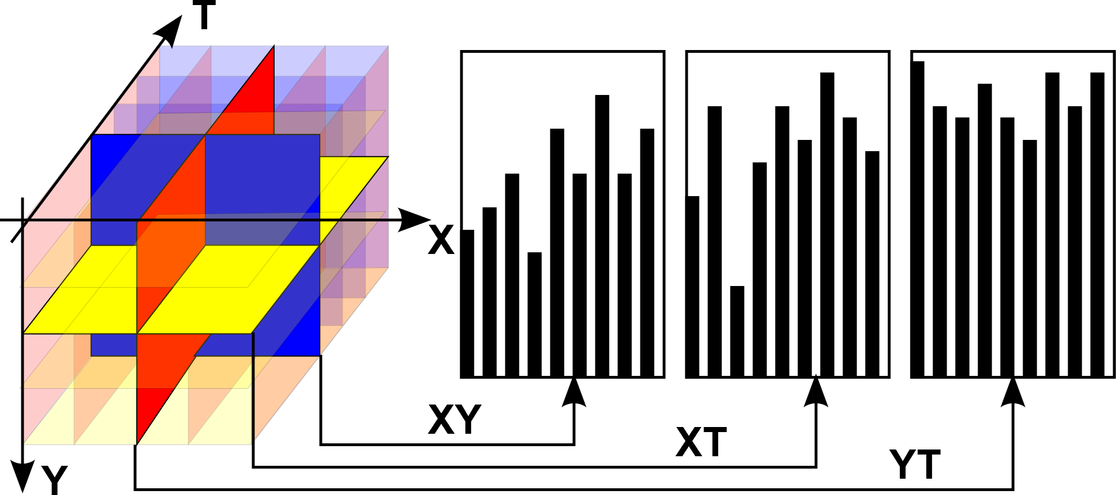
\includegraphics[height=0.1\textheight]{LBPTOP_fig.png}}
  \hspace*{\fill}
  \caption{The different \ac{lbp} descriptors: (a) \ac{lbp} with $(R=2,P=16)$ - (b) \ac{lbptop}~\cite{zhao2012rotation}.}
  \label{fig:lbp}
\end{figure}

\subsection{Feature representation}\label{subsec:fearep}
\todo{give the idea of a single descriptor per volume}

Each \ac{oct} volume can be described by its texture and we employed two strategies.

\begin{description}

\item[Low-level representation] The texture descriptor of an \ac{oct} volume is defined as the concatenation of the \ac{lbp} histograms.
Therefore, for the \ac{lbptop}, the feature descriptor is computed through the concatenation of the \ac{lbp} histograms of the three orthogonal planes and for the \ac{lbp}, the descriptor is defined either through concatenation of the \ac{lbp} histograms per each B-scan (\emph{gocal}-mapping), or per each \ac{sw} (\emph{local}-mapping).\\

\begin{changebar}
  \todo{fab got confused with the Rotation invariant, and would like more detail(or reworking) of the resulting descriptor.}
\added[id=moj]{
\emph{Global} mapping considers to extract the features from the 2D B-scans for \ac{lbp} and 3D volume for \ac{lbptop}.
Therefore for a volume with $d$ B-scans, the \emph{global}-\ac{lbp} feature leads to a final descriptor of size $d \times \ac{lbp}_{hist}$ and \emph{global}-\ac{lbptop} feature returns the final descriptor of size $3 \times \ac{lbp}_{hist}$.
Here $\ac{lbp}_{hist}$ refers to the size of uniform and rotation invariant \ac{lbp} histogram which it's number of bins depends on the number of sampling points in a given neighborhood.
}


\added[id=moj]{
In \emph{local} mapping, the features are extracted from a set of 2D patches for \ac{lbp} and a set of sub-volumes for \ac{lbptop}.
Considering a ($m \times m$) \acf{sw} for 2D \ac{lbp} and ($ m \times m \times m$)  sub-volume for \ac{lbptop}.
Using these elements, the \emph{local}-\ac{lbp} approach provides a final descriptor of size ($d \times N \times \ac{lbp}_{hist}$) while \emph{local}-\ac{lbptop} results in a final descriptor of size $\frac{d}{m} \times N \times 3 \times \ac{lbp}_{hist}$.
Here $N$ is the total number of elements in each B-scan, and 3D volume, respectively.
}\\
\end{changebar}

\item[High-level representation] According to the chosen mapping strategy, the low-level representation can lead to a high dimensional feature space.
High-level representation simplifies this high dimensional feature space into a more discriminant lower space.
\ac{bow} approach is used for this purpose~\cite{Sivic2003}.
This model represents the features by creating a visual dictionary or ``codebook'', from the set of low-level features.
The set of low-level features are clustered using \textit{k}-means to create the codebook with \textit{k} clusters or visual words.
After creating the codebook, each of the training example is represented as a histogram of size \textit{k}.
The histogram is obtained by calculating the frequency of occurrences of each of the \textit{k} words in the extracted features from the training example.
%\Ac{pca} and \ac{bow} among other methods, are used for this purpose~\cite{Sivic2003}.
%Although \ac{pca} maps the data according to their variance, \ac{bow} models represent the features by creating a visual dictionary, or ``codebook'', from the set of low-level features.
%The set of low-level features is clustered using \textit{k}-means to create the codebook with \textit{k} defining the number of visual words.
%After creating the codebook, each of the training example is represented as a histogram of size \textit{k} obtained by calculating the frequency of occurrences of each of the \textit{k} words in the features extracted from the training example.

\end{description}

%\subsubsection{Low-level features} are extracted considering the whole volume using LBP and 3D-LBP descriptors.
% LBP is a discriminative rotation invariant feature descriptor proposed by Ojala et al. \cite{ojala2002multiresolution}.
% LBP descriptor encodes the intensity differences of a central pixel ($g_c$) with its neighboring pixels ($g_{p}$), within in a defined neighborhood of radius $R$. The differences are encoded in terms of binary patterns as in~Eq. \ref{Eq:LBP}:

% \begin{equation} \label{Eq:LBP}
% LBP_{P,R} = \sum_{p=0}^{P-1}s(g_{p} - g_{c})2^{p},
% \end{equation}
% where $s(a) = 1$ if $a \geq 0$, and $s(a)=0$ otherwise. $P$ is the number of sampling points in the circle of radius $R$.

% The binary patterns are calculated for each pixel in the given image and their histogram defines the final descriptor.
% The LBP histograms are computed for each slice of the volume and are concatenated into a single histogram. This forms the first low-level feature.
% The second low-level descriptor is defined in a similar manner as the first one. However principal component analysis (PCA) is applied to the concatenated histograms in order to reduce the dimension.

% For the third low-level descriptor, since the OCT data is a 3D volume, following the approach of Zhao \textit{et al}. \cite{zhao2007dynamic}, we extract 3D-LBP by considering three orthogonal planes, XY, XZ and YZ. Note that $X$, $Y$, and $Z$ are respectively the horizontal, vertical and depth direction of the OCT volume as shown in Figure~\ref{fig:oct_data}(a).
% LBP patterns are computed for each of the three planes, and the obtained three histograms are concatenated into a final 3D-LBP descriptor.



% \subsubsection{High-level features} - are extracted using bag of words (BoW) approach which is a feature representation technique based of creating a visual dictionary, or codebook, from a set of low-level features~\cite{Sivic2003}.
% To do so, the OCT images are divided into local patches and LBP histograms are computed for every local patch.
% This set of LBP histograms is then used to create a codebook using K-means clustering. If we define $K$ clusters in the feature space, then the visual dictionary will contain $K$ words each one being the center of one cluster.
% After creating the codebook, each of the training example is represented as a histogram of size $K$ obtained by calculating the frequency of occurrences of each of the $K$ words in the features extracted from the training example.
% Note that in the 2D case, each slice is divided into patches of size $N\times N$ and we extract 2D-LBP from each patch, while in the 3D case, the volume is divided into $N \times N \times N$ patches and 3D-LBP histograms are computed. In our experiments in Section 3, we set $N=7$, and vary the size of the codebook $K$ in the range $\{2, 4, 8, 16, 32, 64, 100 \}$.
% % \tikzstyle{block} = [rectangle, draw, fill=gray!20, text = black,
    text width=6em, text centered, rounded corners, minimum height=4em , minimum width = 6em]
    % \tikzstyle{line} = [draw, -latex']
  \tikzstyle{myarrow}=[->, thick]
    \tikzstyle{line}=[-, thick]
    \tikzstyle{block2} = [rectangle, draw, fill=white!20,
    text width=6em, text centered, rounded corners, minimum height=4em, minimum width = 6em]
    \tikzstyle{block3} = [rectangle, draw, fill=gray!20, text = black,
    text width=7em, text centered, rounded corners, minimum height=4em , minimum width = 7em]
\def\blockdist{1}
\def\edgedist{1.5}
  %%%% The Framework Sparse Coding 

\begin{figure}
 \begin{center}
   \begin{tikzpicture}[node distance = 1cm,scale=0.6, every node/.style={scale=0.6}]
%(FEx.east|- FEx.south)
    \node [block2] (input) {Training image};
    %\node [block, right of = input, node distance = 2.8cm](Seg){Segmentation}; 
    \node [block, right of=input,node distance = 2.8cm](De){Denoising};
    \node [block, right of=De,node distance = 2.8cm](FEx){Feature extraction};
    \path (FEx.east)+(+0.8,0) node (g) {};
    
    %%% Sparse Coding Block
    \node [block3, right of=g,node distance = 1.7cm](DL){Dictionary learning /k-means};
    \node [block3, below of=DL,node distance = 2.5cm](PR){Projection};
    \begin{pgfonlayer}{background}
      \path (DL.west |- DL.north)+(-0.4,-0.1+\blockdist) node (a) {};
      \path (PR.east |- PR.south)+(+0.4,-0.7) node (b) {};          
      \path[fill=gray!10,rounded corners, draw=gray!20, dashed] (a) rectangle (b);
    \end{pgfonlayer}
\path (DL.west |- DL.north)+(+1.2,-0.5+\blockdist) node (SP) {\textbf{Bag of Features}};
\path (PR.east |- PR.south)+(-1.3,-0.4+\blockdist) node (c){};
\path (PR.east)+(-3.15,0) node (d) {};

%%% Testing 
\node [block, below of=FEx, node distance = 2.5cm](FE2){Feature extraction};
\node [block, below of=De, node distance = 2.5cm](De2){Denoising};
% \node [block, below of=Seg, node distance = 2.5cm](Seg2){Segmentation}; 
\node [block2, below of=input, node distance = 2.5cm](TestImg){Testing image};

%%% 
\node [block, right of=PR, node distance = 3.6cm](Pool){Visual words histogram};
\path (Pool.east) + (0.3,0) node (f){}; 
\path (Pool.east) + (0.2,-0.1) node (f1){}; 

%%% Classification
\node [block, right of = Pool, node distance = 3.5cm] (Pre){Prediction}; 
    \node [block, above of = Pre, node distance = 2.5cm] (Learn){Learning}; 
    \begin{pgfonlayer}{background}
      \path (Learn.west |- Learn.north)+(-0.4,-0.1+\blockdist) node (h) {};
    \path (Pre.east |- Pre.south)+(+0.4,-0.7) node (i) {};          
    \path[fill=gray!10,rounded corners, draw=gray!20, dashed] (h) rectangle (i);
\end{pgfonlayer}
\path (Learn.west |- Learn.north)+(+1.1,-0.5+\blockdist) node (Clas) {\textbf{Classification}};
\path (Pre.east |- Pre.south)+(-1.3,-0.4+\blockdist) node (j){};
\path (f1.north)+(0, 2.5) node (k) {};
\path (Pre.east) + (1.2,0) node (k1) {P(..)}; 

    % Draw edges
    \draw [line] (input) -- (De) -- (FEx); 
    \draw [myarrow] (FEx)-- (DL);
    \draw [myarrow] (DL) -- (PR) ; 
    \draw [line] (TestImg) -- (De2) -- (FE2); 
    \draw [myarrow] (FE2) -- (PR) ;
    \draw [line] (PR) -- (Pool); 
    \draw [myarrow] (Pool) -- (Pre); 
    \draw [line] (f1.north) -- + (0,2.5)(k.south); 
    \draw [myarrow] (k.south)+ (0,0.1)  -- (Learn.west); 
    \draw [myarrow] (Pre) -- (k1);

    \end{tikzpicture}
    \end{center}
    

\caption{Bag of features framework} 
\label{fig:BoF-framework}

\end{figure}

\subsection{Classification}\label{subsec:cls}
% Classification is a supervised learning method which intends to find a mapping $f(.)$ which relates a set of input $x$ to a set of categorical outputs $y$.
% The learning is comprehended using a training set, which contains a set of $N$ samples with their associated labels~\cite{murphy2012machine}.

Classification corresponds to the mapping of a set of inputs $\mathbf{x}$ into a set of categorical outputs $\mathbf{y}$ using a linear or non-linear function $f(\cdot)$.
In supervised learning methods, this function is defined by providing a training set of $N$ samples $\mathbf{x}_{tr}$ with their associated labels $\mathbf{y}_{tr}$.
In the remainder of this section, we briefly summarize the supervised classification methods used in the experiments.

\begin{description}

\item[$k$-\acf*{nn}] is a non-parametric classification method in which an unlabeled feature vector $x$ is assigned to the majority class of its $k$ nearest-neighbors from the training set.
To avoid a tie case, the parameter $k$ is set to an odd number.\\

\item[\acf*{lr}] is a linear classifier which uses the logistic function to estimate the probability of $x$ to belong to a particular class $c_i$~\cite{cox1958regression}.
Thus, the posterior probability is expressed as:
\begin{equation} \label{eq:ppc1lr}
p(c_{i}|x) = \frac{1}{1+\exp(-w^{T}x)}
\end{equation}
\noindent where $w$ is a vector of the regression parameters to obtain a linear combination of the input feature vector $x$.
Using this model the unlabeled sample is assigned to the class which maximizes the posterior probability.
\begin{equation}
C(x_{i}) =  \text{arg}\max\limits_{k} p(C = k| x_{i})
\end{equation}
In this method, finding an optimal set of parameters for $w$ is essential.
The vectors of parameters $w$ can be inferred by finding the maximum likelihood estimates via optimization methods such as quasi-Newton method~\cite{byrd1994representations}.\\

\item[\acf*{rf}] is an ensemble of decision trees and was introduced by~\cite{breiman2001random}.
The ensemble uses each tree to predict an output and finalizes the ultimate prediction by aggregating the outputs of all tress.
This classifier learns the data by training multiple decision trees on bootstrap samples of the original data.
Each bootstrap of $D$ dimension is used for training one decision tree and at each node, the best split among randomly ($d << D$) selected subset of descriptors is chosen.
Each tree is grown to its maximum length without any pruning.
In the prediction stage a sample is voted by each tree and it is labeled by considering the majority of the votes.\\
%% Another explanation from BIOIMAGING:
%is an ensemble of decision trees~\cite{breiman2001random} which generalizes the classification process by applying two types of randomization: at the tree level, each tree is fed by a bootstrap made of $S'$ samples which are built from the original data of size $S$ such that  $S=S'$, and at the node level, a subset of feature dimensions $m$ is randomly selected from the original dimension $M$ such that $m=\sqrt{M}$.
%The trees in \ac{rf} are grown to their maximum length without any pruning.
%Figure~\ref{fig:rftrain} shows the training stage of \ac{rf} ensemble.
%In the testing stage, each tree in the ensemble casts a unit vote in the final prediction and the final prediction is based on combination of all the votes.

\item[\acf*{gb}] is a generalization form of \ac{adb}, which is able to use real-value weak learners and minimizes different loss functions~\cite{zheng2007general}.
\ac{gb} builds the ensemble in a greedy manner.
It iteratively selects the best pair of real-valued weak learners and adjust their weights so that they minimize a given differentiable loss function.
%\begin{subequations}
%\begin{align}
%\varphi(x) & = \sum\limits_{j = 1}^{M} \alpha_{j} h_{j}(x)\\
%\mathcal{L} & = \sum\limits_{i = 1}^{N} L(y_{i}, \varphi(x_{i}))
%\end{align}
%\end{subequations}
%\noindent Here $h_{j}(.)$ is the weak learner and $\alpha_{j}$ is the real value weight and the aim is to minimize $\mathcal{L}$.
Common choice for the weak learner is decision stumps or regression trees while the loss function is generally an exponential loss or a logarithmic loss~\cite{becker2013supervised}.
%\begin{subequations}
%\begin{align}
%\text{Exponential loss } \qquad L &= e^{-y_{i}\varphi(x_{i})} \label{eq:exploss} \\
%\text{Log loss } \qquad L &= \log(1+e^{-2y_{i}\varphi(x_{i})})
%\end{align}
%\end{subequations}
This minimization is carried out via gradient descent or quadratic approximation.\\

\item[\acf*{svm}]~\cite{vapnik1963generalized} is a sparse kernel method which aims to separate two classes by finding the best hyperplane which maximizes the margin between the two classes.
Maximizing the margin is equivalent to minimizing the norm of the normal vector of the hyperplane:
\begin{equation}
\min\limits_{\mathbf{w}, \omega_{0}} \frac{1}{2} \Vert \mathbf{w}\Vert^{2} \qquad \text{s.t. } \quad  y_{i}(\mathbf{w}^{T}\mathbf{x_{i}} + \omega_{0}) \geq 1, i = 1: N
\label{eq:svmsm}
\end{equation}
\noindent This constraint intends to force all the point to be in the correct side of the decision boundary (hyperplane) with a minimum distance of 1.
This assumption is only valid if the data is linearly separable.
Thus for general cases a slack variable $\xi_{i} \geq 0 $ is introduced, which is $\xi_{i} = 0 $, if the points are on/or inside the correct margin boundary, is $0 < \xi_{i} \leq 1 $ if the points are inside the margin but in the correct side of the decision boundary and otherwise if they lie in the wrong side of decision boundary is $\xi_{i} > 1 $.
This assumption introduces the \textit{soft margin constraints}.
Therefore the optimization problem of \ac{svm} classifier is presented by:

\begin{align}
 & \min\limits_{\mathbf{w},\omega_{0}, \mathbf{\xi}} \frac{1}{2} \Vert \mathbf{w} \Vert^{2} + C \sum\limits_{i = 1}^{N} \xi_{i} \nonumber \\
\text{s.t. } & \quad \xi_{i} \geq 0, \quad y_{i}(x_{i}^{T}\mathbf{w} + \omega_{0}) \geq 1 - \xi_{i}, i = 1:N
\label{eq:svmop}
\end{align}
In Eq.~\ref{eq:svmop}, the $\sum_{i} \xi_{i}$ term, describes the upper bound on the number of misclassified points and $C$ is the regularization parameter that controls the tolerance of the classifiers on the number of errors~\cite{murphy2012machine}. \\

\end{description}


% Random Forest


%%% Local Variables:
%%% mode: latex
%%% TeX-master: "../../main.tex"
%%% End:
